% Archivo generado automáticamente con los problemas
\section*{Problems}
Sección: 36_Jets_and_effective_field_theory
Páginas: 829-831
Contenido:
36.1 Show that in the dijet region τ ≈τ1. In particular, show that the singular terms in
dσ
dτ are the same as the singular terms in dσ
dτ! for any number of particles.

36.2 Collinear factorization.
(a) Show that the collinear factorization in Eq. (36.51) holds for multiple emissions
in scalar QED.
(b) Show that the collinear factorization in Eq. (36.43) holds for multiple emissions
in QCD.

36.3 Calculate the g →gg splitting function from the matrix element of gluon jet fields
following the approach in Section 36.4.2. Average over azimuthal angle, you should
find Pgg = 2CA

z
1−z + 1−z
z
+ z(1 −z)

, as in Eq. (32.54).

36.4 Show soft-collinear factorization at leading power for two emissions in scalar QED.
That is, show that
⟨Ω|φ⋆
1φ2|p1p2; q; k⟩∼⟨Ω|φ⋆
1W1|p1; q⟩⟨Ω|W †
2 φ2|p2⟩⟨Ω|Y1Y †
2 |k⟩,
(36.135)
where pμ
1 and pμ
2 are the momenta of the scalars, kμ is the momentum of a soft
photon and q is the momentum of a photon collinear to p1.

36.5 Calculate the quark self-energy graph at 1-loop in lightcone gauge. Show that the
imaginary part gives the same jet function as computed in Section 36.6.2.

36.6 Threshold Drell–Yan.
(a) Show that near partonic threshold, the Drell–Yan cross section can be written as
dσ
dM 2 =
4πα2Q2
q
3NM 2√s|C|2
 dξ1
ξ1
dξ2
ξ2
f(ξ1) f(ξ2) ˆWDY
√s(1 −z)

, (36.136)
where
ˆWDY(ω) =

dt
4π e
i
2 ωx0WDY

x0,⃗0

.
(36.137)
(b) Compute the Wilson coefficient C for Oμ in Eq. (36.73) at order αs.
(c) Calculate WDY(x) and ˆWDY(ω) to 1-loop.
Problems
811

36.7 Laplace transforms are extremely useful for solving RGEs in SCET. We define the
Laplace transform of a function f(τ) as
˜f(ν) ≡
 ∞
0
dτe−ντf(τ).
(36.138)
(a) Show that the cross section in Eq. (36.101) simplifies to
˜σ(ν) = H˜j(ν)2˜sT (ν)
(36.139)
in Laplace space.
(b) Show that the RGE for the jet function in Eq. (36.127) simplifies to
μ d
dμ
˜j(ν, μ) = αs(μ)
−2ΓJ ln
Q2
eγEνμ2 −2γJ
˜j(ν, μ) .
(36.140)
What are ΓJ and γJ? Find a similar RGE for the Laplace-transformed soft
function.
(c) Solve the RGE for the jet function in Laplace space and show that the result, in
position space, is as in Eq. (36.128).

36.8 Sukakov RGEs.
(a) Verify that Eq. (36.124) solves Eq. (36.123).
(b) Show that the function S(ν, μ) in Eq. (36.126) has the expansion
S(ν, μ) =
πCF
β2
0αs(ν)
1 −αs(μ)
αs(ν) −ln αs(μ)
αs(ν) + O(αs)
.
(36.141)
(c) Find a similar expansion for AH(ν, μ).

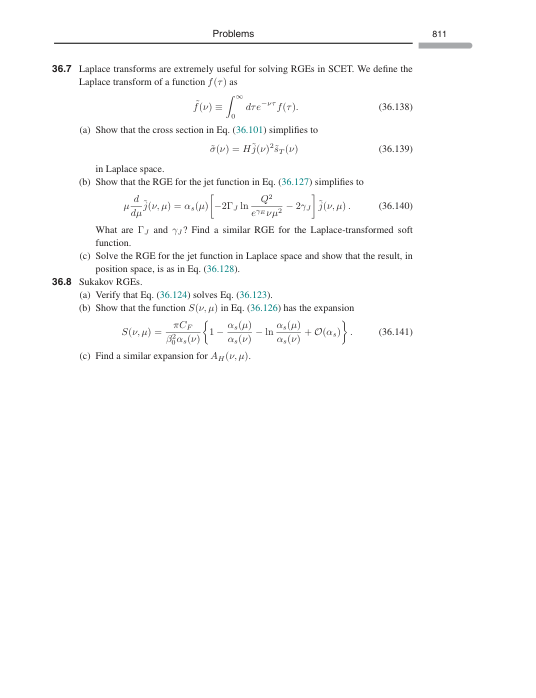
\includegraphics{./figs/36_Jets_and_effective_field_theory_page_831.png}

---

